%%% LaTeX Template: Article/Thesis/etc. with colored headings and special fonts
%%%
%%% Source: http://www.howtotex.com/
%%% Feel free to distribute this template, but please keep to referal to http://www.howtotex.com/ here.
%%% February 2011
%%%
%%% Modified January 2016 by CDM

%%%  Preamble
\documentclass[11pt,letterpaper]{article}
\usepackage[margin=1.0in]{geometry}
\usepackage[T1]{fontenc}
\usepackage[bitstream-charter]{mathdesign}
\usepackage[latin1]{inputenc}					
\usepackage{amsmath}						
\usepackage{xcolor}
\usepackage{cite}
\usepackage{hyphenat}
\usepackage{graphicx}
\usepackage{float}
\usepackage{subfigure}
\usepackage{sectsty}
\usepackage[compact]{titlesec} 
\usepackage[tablegrid]{vhistory}
\usepackage{pbox}
\allsectionsfont{\color{accentcolor}\scshape\selectfont}

%%% Definitions
\definecolor{accentcolor}{rgb}{0.0,0.0,0.5} 
\newcommand{\teamname}{Robo Crew}
\newcommand{\productname}{RV8 Workcell}
\newcommand{\coursename}{CSE 4317: Senior Design II}
\newcommand{\semester}{Spring 2024}
\newcommand{\docname}{Architectural Design Specification}
\newcommand{\department}{Department of Computer Science \& Engineering}
\newcommand{\university}{The University of Texas at Arlington}
\newcommand{\authors}{Akshay Paluri \\ Ameen Mahouch \\ Muhammad Anas \\ Hyun Ho Kim\\ Kundan Singh Mahato}

%%% Headers and footers
\usepackage{fancyhdr}
	\pagestyle{fancy}						% Enabling the custom headers/footers
\usepackage{lastpage}	
	% Header (empty)
	\lhead{}
	\chead{}
	\rhead{}
	% Footer
	\lfoot{\footnotesize \teamname \ - \semester}
	\cfoot{}
	\rfoot{\footnotesize page \thepage\ of \pageref{LastPage}}	% "Page 1 of 2"
	\renewcommand{\headrulewidth}{0.0pt}
	\renewcommand{\footrulewidth}{0.4pt}

%%% Change the abstract environment
\usepackage[runin]{abstract}			% runin option for a run-in title
%\setlength\absleftindent{30pt}			% left margin
%\setlength\absrightindent{30pt}		% right margin
\abslabeldelim{\quad}	
\setlength{\abstitleskip}{-10pt}
\renewcommand{\abstractname}{}
\renewcommand{\abstracttextfont}{\color{accentcolor} \small \slshape}	% slanted text

%%% Start of the document
\begin{document}

%%% Cover sheet
{\centering \huge \color{accentcolor} \sc \textbf{\department \\ \university} \par}
\vspace{1 in}
{\centering \huge \color{accentcolor} \sc \textbf{\docname \\ \coursename \\ \semester} \par}
\vspace{0.5 in}
\begin{figure}[h!]
	\centering
   	
\includegraphics[width=0.60\textwidth]{images/robocrew.jpg}
\end{figure}
\vspace{0.5 in}
{\centering \huge \color{accentcolor} \sc \textbf{\teamname \\ \productname} \par}
\vspace{0.5 in}
{\centering \large \sc \textbf{\authors} \par}
\newpage


%\vspace{1 in}
%\centerline{January 13th, 2012}
%\newpage

%%% Revision History
\begin{versionhistory}
  	\vhEntry{0.1}{02.12.2024}{AM, MA, AP, HK, KM}{document creation}
\end{versionhistory}
\newpage

%%% Table of contents
\setcounter{tocdepth}{2}
\tableofcontents
\newpage

%%% List of figures and tables (optional)
\listoffigures
\listoftables
\newpage

%%% Document sections
\section{Introduction}
This product is a high level working prototype of an industrial level robot which serves the purpose of ordering and arranging the boxes by scanning the QR codes. The boxes will be picked by a gripper (custom designed) and will be sorted. The robot arm is connected to a PLC controller and the arm is set on to an additional axis (i.e. linear rail) which is also connected to a servo amplifier present in the PLC. This PLC controller is connected to a PC containing various software to control the robot arm. Raspberry Pi is used for the QR code detection and decision making which is connected to a camera.
\section{System Overview}
This section defines the top-level logical view of the design and describes the detail architectural strategy for the RV8 work cell system flow. Three separate layers make up the structure of the system: input, processing, and output. With the help of these layers, which are all essential to the system, the robot is able to carry out dynamic tasks that are dependent on the processing of sensor data. A high-level block diagram that shows the connections and interactions between different layers is included in this part to provide readers a thorough understanding of the architecture of the entire system. A robotic system's input layer, which makes use of sensors like a gate sensor and an E-stop is essential for task execution. E-stops offer an emergency shutdown signal that allows the system to be stopped right away. The robot arm's speed is controlled by the Gate sensor, which also communicates with the controller to find out the cage gate's present state. Efficiency and safety are prioritized in this design, which allows the robot to respond and adapt to a variety of scenarios while integrating security features like gate status monitoring and emergency stops. With the integration of sensors will perform the operation such as splashing multi-color paint to the desire target with great level of precision. PC and the trigger switch will be inter-connected to the PC to perform the necessary communication to perform the given task.  

\begin{figure}[h!]
	\centering
 	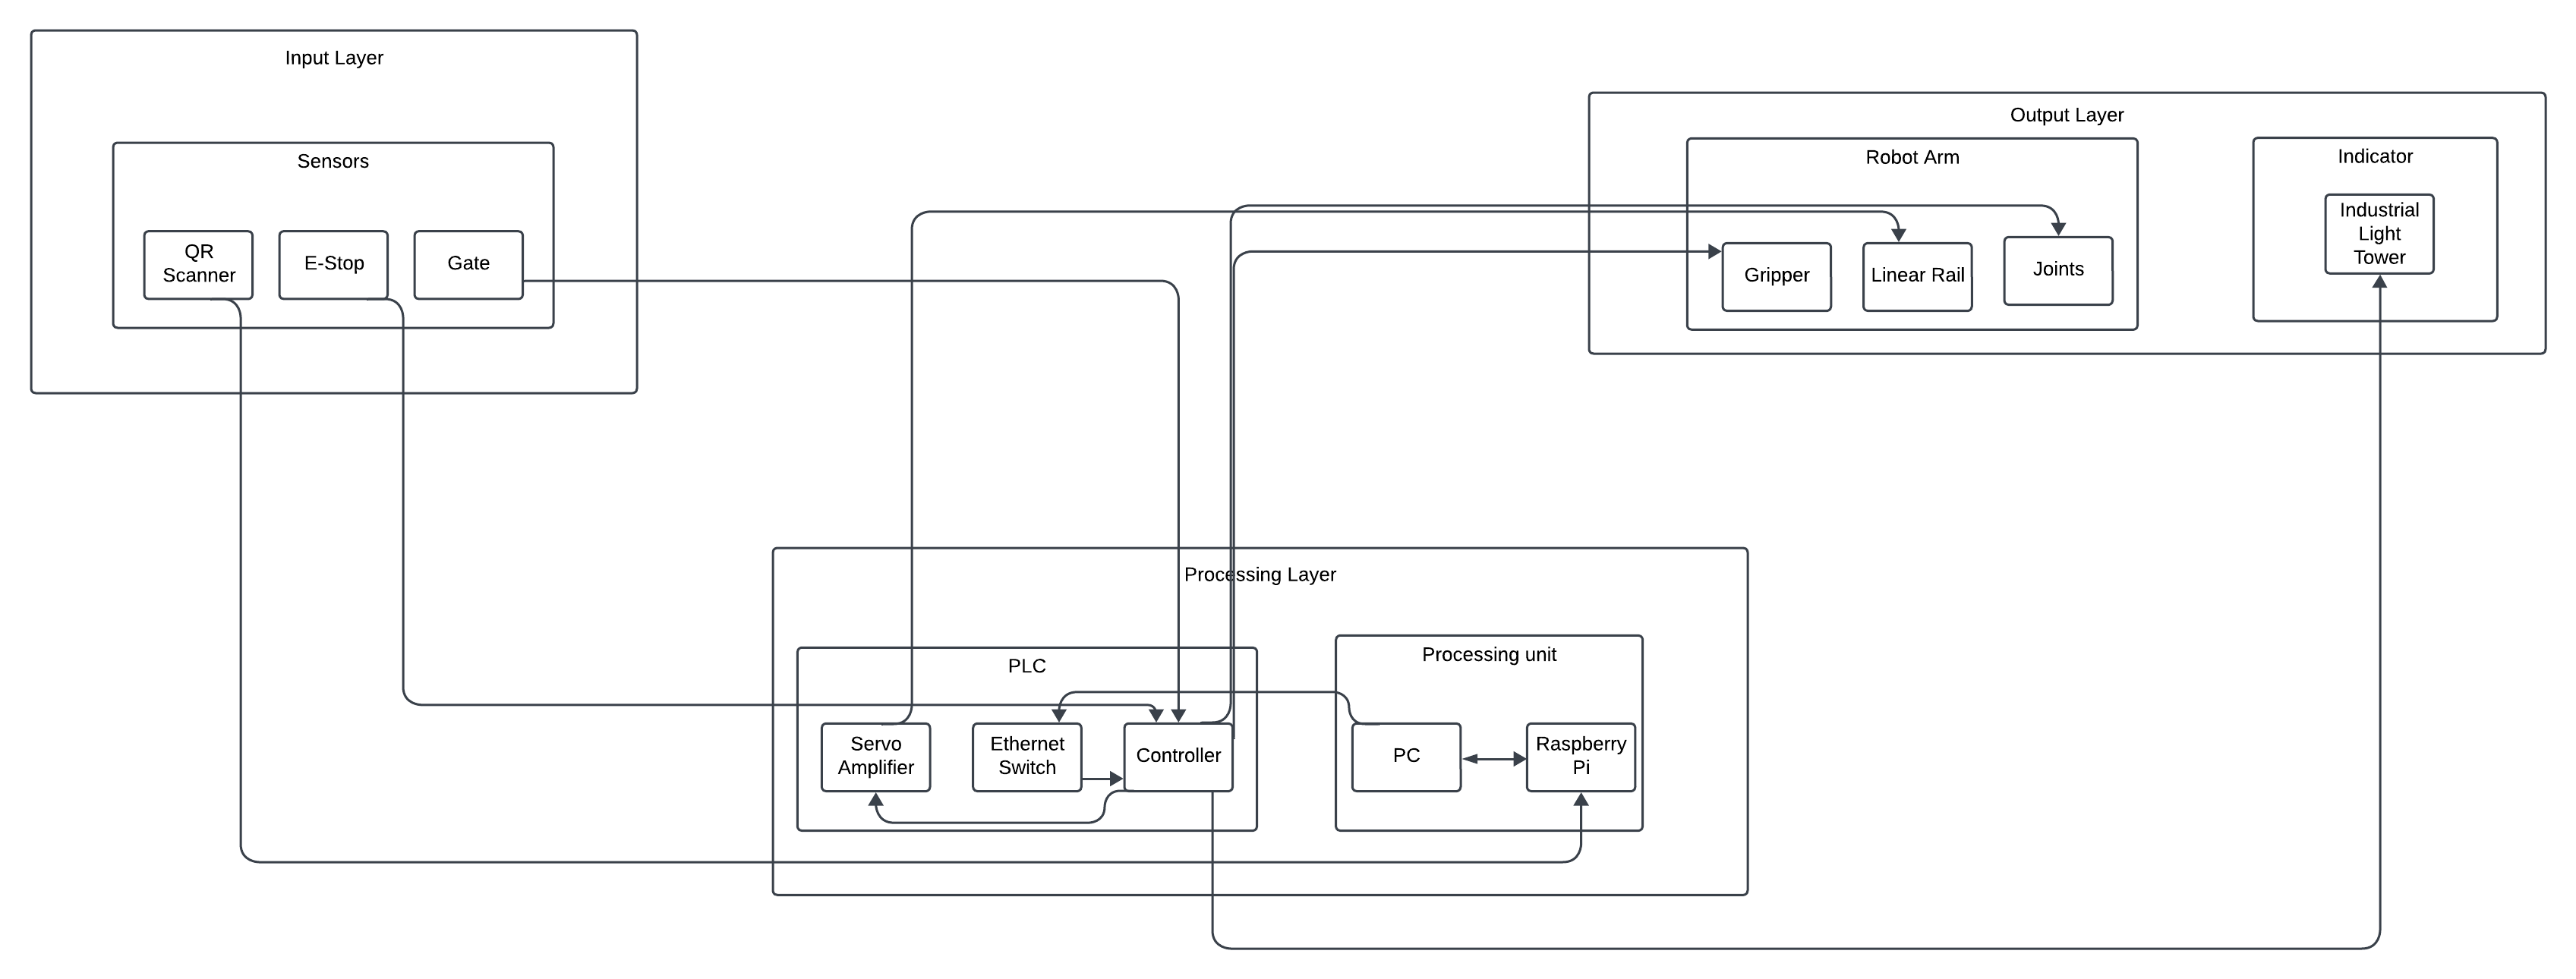
\includegraphics[width=1\textwidth]{images/system_subystem.png}
 \caption{System architecture}
\end{figure}

\newpage
%\section{Subsystem Definitions \& Data Flow}
%This section breaks down your layer abstraction to another level of detail. Here you grapically represent the logical subsytems that compose each layer and show the interactions/interfaces between those subsystems. A subsystem can be thought of as a programming unit that implements one of the major functions of the layer. It, therefore, has data elements that serve as source/sinks for other subsystems. The logical data elements that flow between subsystems need to be explicitly defined at this point, beginning with a data flow-like diagram based on the block diagram.

\begin{figure}[h!]
	\centering
 	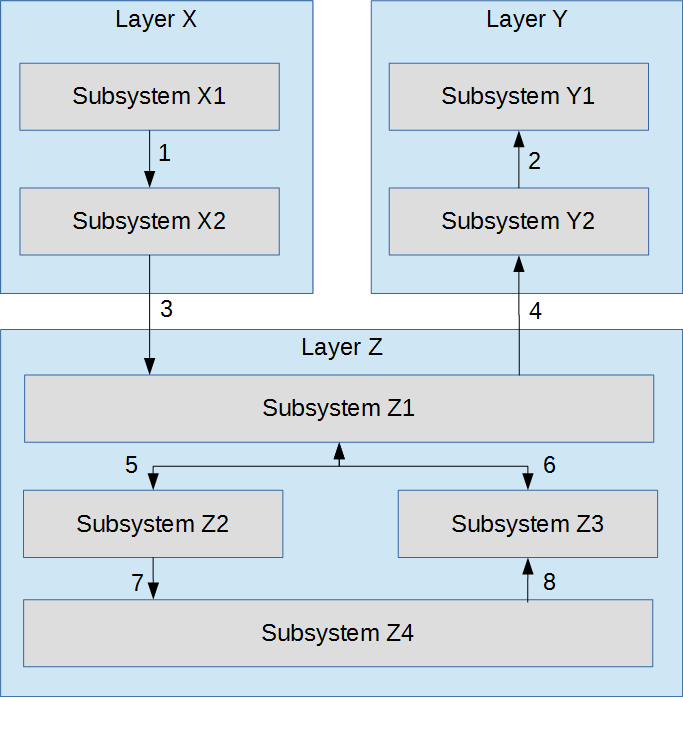
\includegraphics[width=\textwidth]{images/data_flow}
 \caption{A simple data flow diagram}
\end{figure}

\newpage
\section{Input Layer Subsystems}
The input layer plays an important part in executing the spray painting task as per the programmed movement. The input in this system comes from the host PC and the sensors. The host PC acts as a centralized location to write programs for robotic movement, as well as control PLC logic. The sensors involved in the system are emergency stops (e-stops) and inductive switches. These inputs send signals to the PLC on particular situations and scenarios to keep the safety measure intact. Inductive switches make sure that the robot arm is calibrated properly before it executes its task. Where as emergency stops immediately halt the robot's operation, ensuring the safety of personnel and preventing potential accidents.


\subsection{Layer Hardware}
The sensors, including e-stops and inductive switches are the layer hardware for the input layer. 
%The sensors, including the vision sensor, e-stops, and gate, are connected to the programmable logical controller (PLC) via wires. They continuously transmit input values to the PLC, enabling the system to make informed decisions about subsequent actions.

\subsection{Layer Operating System}
Operating system used for this is Windows 10.
%RT ToolBox 3 Pro can be installed on both Windows 11 and Windows 10 operating systems.

\subsection{Layer Software Dependencies}
RT Toolbox is required.
%RT ToolBox 3, which controls the robot, will be used to facilitate the movement of the robot arm.

\subsection{E-Stops}
There will be multiple emergency stop (E-stop) buttons strategically placed throughout the system. These buttons will be located next to the case gate, on the controller, and inside the cage. When any of these e-stop buttons are pressed, the entire system will immediately halt, ensuring rapid response to any safety concerns or emergencies.


\begin{figure}[h!]
	\centering
 	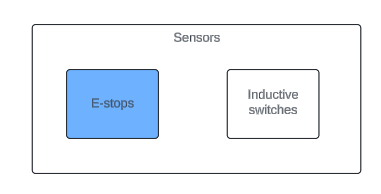
\includegraphics[width=0.60\textwidth]{images/E_stop_sensor.png}
 \caption{Sensor subsystem diagram}
\end{figure}

\subsubsection{Subsystem Hardware}
2 wired emergency stops connected to the CNUSR11 connector of the controller. 1 emergency stop located on the controller.

\subsubsection{Subsystem Operating System}
N/A

\subsubsection{Subsystem Software Dependencies}
N/A

\subsubsection{Subsystem Programming Languages}
N/A

\subsubsection{Subsystem Data Structures}
N/A

\subsubsection{Subsystem Data Processing}
The signals are send through wires to robot controller for processing to halt the robot.

\subsection{Inductive Switches}
Inductive switches are placed on the edges of linear rail to mark the endpoints. Using these switches will help the robot to calibrate the center of linear rail whenever robot starts.

\begin{figure}[h!]
	\centering
 	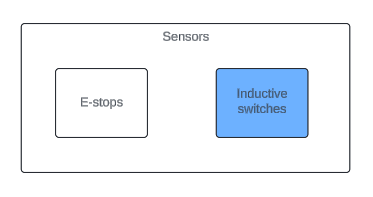
\includegraphics[width=0.60\textwidth]{images/Inductive_sensors.png}
 \caption{Sensors subsystem diagram}
\end{figure}

\subsubsection{Subsystem Hardware}
The inductive proximity sensor is a barrel-type sensor with PNP output, featuring a 1.5mm sensing range. It operates with a 3-wire configuration and is rated IP67. These sensors are typically connected to the general-purpose input/output pins of the PLC.%Inductive Proximity Sensors are used to limit the range of movement of the robot arm along the X-axis, E-stop sensors are utilized for emergency situations (True/False), and wires are employed to connect them to the PLC.

\subsubsection{Subsystem Operating System}
Windows 10.

\subsubsection{Subsystem Software Dependencies}
GX Works is needed in order to write ladder logic that processes the signals to act appropriately.

\subsubsection{Subsystem Programming Languages}
MELFA-BASIC VI programming language.

\subsubsection{Subsystem Data Structures}
N/A

\subsubsection{Subsystem Data Processing}
The switch sends a signal to the PLC when the robot passes over it. 

\subsection{RT Toolbox}
The RT Toolbox is a software package developed by Mitsubishi Electric for their industrial robots. It serves as a comprehensive toolset to assist with various tasks related to robot programming, configuration, and maintenance

\begin{figure}[h!]
	\centering
 	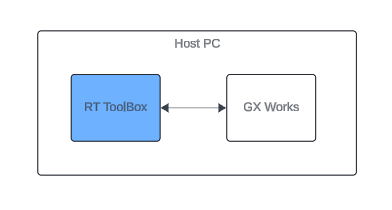
\includegraphics[width=0.60\textwidth]{images/RT_toolbox_Host.png}
 \caption{Host PC subsystem diagram}
\end{figure}

\subsubsection{Subsystem Hardware}
Host PC acts as system hardware in which RT Toolbox operates.

\subsubsection{Subsystem Operating System}
Windows 10.

\subsubsection{Subsystem Software Dependencies}
N/A

\subsubsection{Subsystem Programming Languages}
MELFA BASIC VI.

\subsubsection{Subsystem Data Structures}
Synchronous execution of the code.

\subsubsection{Subsystem Data Processing}
Utilizing Host PC's memory.

\subsection{GX Works}
GX Works3 is the configuration software for FX, L, and Q Series controllers developed by Mitsubishi Electric. GX Works3  interfaces with the work cell's programmable logic controller to program in several languages like ladder logic.

\begin{figure}[h!]
	\centering
 	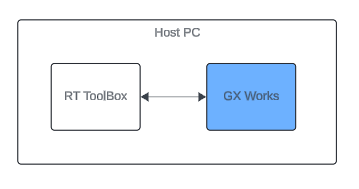
\includegraphics[width=0.60\textwidth]{images/GX_Works_Host.png}
 \caption{Host PC subsystem diagram}
\end{figure}

\subsubsection{Subsystem Hardware}
Host PC acts as system hardware.

\subsubsection{Subsystem Operating System}
Windows.

\subsubsection{Subsystem Software Dependencies}
N/A

\subsubsection{Subsystem Programming Languages}
Ladder Diagram (LD): A graphical representation of relay logic. \\
Structured Text (ST): A high-level textual language based on Pascal. \\
Function Block Diagram (FBD): A graphical language using function blocks. \\
Instruction List (IL): A low-level textual language. \\
Sequential Function Chart (SFC): A graphical language for sequential control.

\subsubsection{Subsystem Data Structures}
N/A

\subsubsection{Subsystem Data Processing}
Using Host PC's memory.
\newpage
\section{Processing Layer Subsystems}
In this section, the processing layer's hardware and software design are delineated. The layer comprises a PLC, Raspberry Pi, and a PC interconnected to facilitate communication and decision-making processes. The PLC primarily governs the robotic arm's movements, including all joints and an additional axis, typically a linear rail. Conversely, the Raspberry Pi is tasked with data collection and transmission to the PC for decision-making regarding task execution on incoming objects, typically boxes. Communication between the PC and PLC ensures alignment of all arm joints for task performance. This section delves into implementation details, covering hardware components, programming languages, software dependencies, and operating systems relevant to the processing layer. Unnecessary details, such as purely software modules without specific hardware components, are omitted for conciseness. Adjustments to the organization, titles, and content are permissible to suit the project's requirements.


\subsection{Layer Hardware}
The hardware involved with the processing layer include a MELSEC Programmable Logic Controller, issued by Mitsubishi. The PLC is a specialized computer used in industrial automation and is paired with software to make decisions based on sensor data like temperature, pressure, or motor position. Finally, the PLC is equipped with an ethernet switch that enables communication between the Host PC and PLC.
\subsection{Layer Operating System}
The operating systems required by the layer are dependent on the specific components. The PLC runs a real-time operating system (RTOS), while the Raspberry Pi utilizes a Linux-based operating system Raspbian, and the host PC runs Windows 10.


\subsection{Layer Software Dependencies}
There are currently no software dependencies.
\subsection{Host PC}
The host PC acts as a powerful processing unit for in-depth analysis, decision making, and control. It receives pre-processed data from the Raspberry Pi, including data from the QR code, and it performs trajectory planning and higher level decision making.

\begin{figure}[h!]
	\centering
 	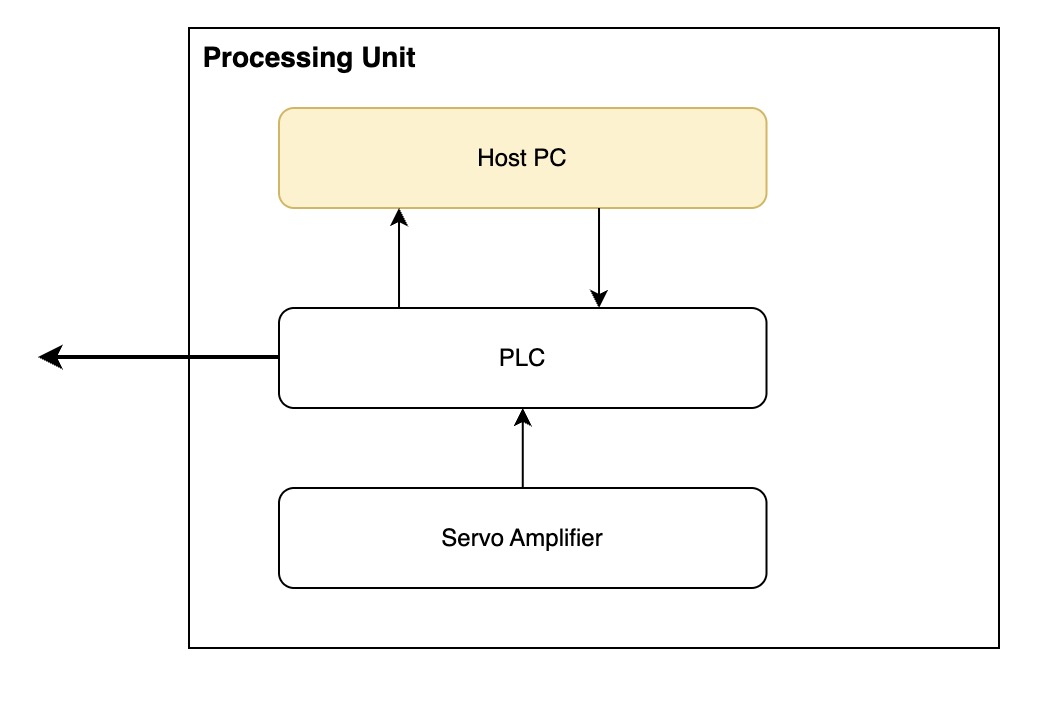
\includegraphics[width=0.6\textwidth]{images/HostPC.jpg}
 \caption{Host PC Subsystem}
\end{figure}

\subsubsection{Subsystem Hardware}
This subsystem consists of a Dell desktop computer with USB connections to the RV-8CRL controller. 
\subsubsection{Subsystem Operating System}
The PC runs Windows 10.
\subsubsection{Subsystem Software Dependencies}
The PC runs several software for the system including RT ToolBox3, GXWorks, MRConfigurator2, and Creality.
\begin{itemize}
    \item RT ToolBox is a software developed by Mitsubishi used for visual programming of the robotic arm, acting as a 3D simulator.
    \item GXWorks is a software suite provided by Mitsubishi Electric for programming and configuring PLCs. It is a comprehensive development environment that supports various programming languages such as ladder logic, function block diagrams (FBD), and structured text (ST).
    \item MRConfigurator2 is a software tool used for programmign Mitsubishi's servo drives and motion controllers.
    \item Creality is used for 3D modeling and design. Primarily, this software is used for designing mechanical components.
\end{itemize}

\subsubsection{Subsystem Programming Languages}
The Host PC uses Python scripts for network communication. The RT ToolBox software supports MELFA-BASIC-VI programming language.

\subsubsection{Subsystem Data Processing}
Upon receiving preprocessed data from the Raspberry Pi, the Host PC engages in thorough data analysis. This includes examining sensor data performing image processing if necessary. Algorithms for noise reduction, edge detection, and image segmentation may be employed to extract relevant information from sensor readings or images. The Host PC manages communication with the PLC using Ethernet/IP. Data packets are assembled and parsed according to the protocol specifications, ensuring reliable and efficient data exchange between the PC and the PLC.

\subsection{Additional Axis Servo}
This subsystem focuses on controlling the additional axis, such as a linear rail, to facilitate precise movements of the robotic arm.
\begin{figure}[h!]
	\centering
 	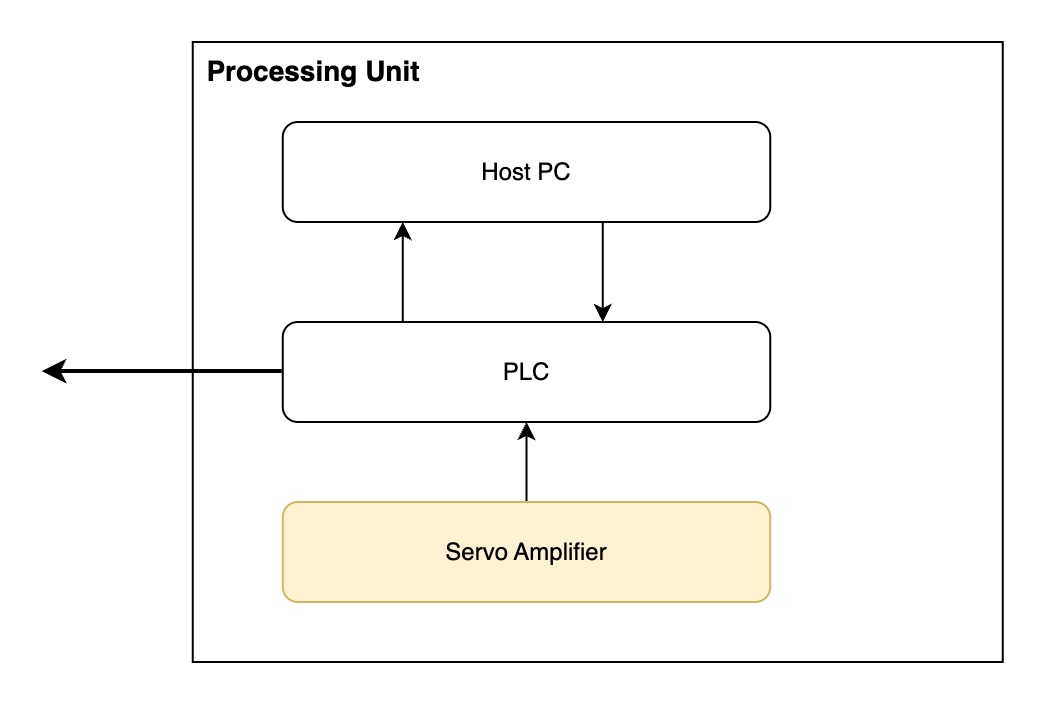
\includegraphics[width=0.65\textwidth]{images/ServoAmp.jpg}
 \caption{Servo Subsystem}
\end{figure}

\subsubsection{Subsystem Hardware}
The subsystem consists of a RollOn linear axis on a Megadyne belt. The servo amplifier is a MELSERVO MR-J4 series. Connections between the servo amplifier and PLC occur through a USB-A.
\subsubsection{Subsystem Software Dependencies}
Servo amplifier parameters are dependent on MRConfigurator2, where they can be specified through read/write operations.

\subsubsection{Subsystem Data Processing}
The servo amplifier receives control signals from the controller and translates them into precise voltage and current outputs to drive a servo motor. It continuously monitors feedback from sensors to maintain accurate motor position and velocity, adjusting operation as needed to minimize discrepancies. Additionally, servo amplifiers incorporate safety features to prevent damage and ensure safe operation of the motor system.


\subsection{Programmable Logic Controller}
The PLC acts as the central component of the processing layer, responsible for coordinating and executing control tasks for the robotic arm and additional axis. This subsection outlines the hardware, software, and data processing aspects specific to the PLC.
\begin{figure}[h!]
	\centering
 	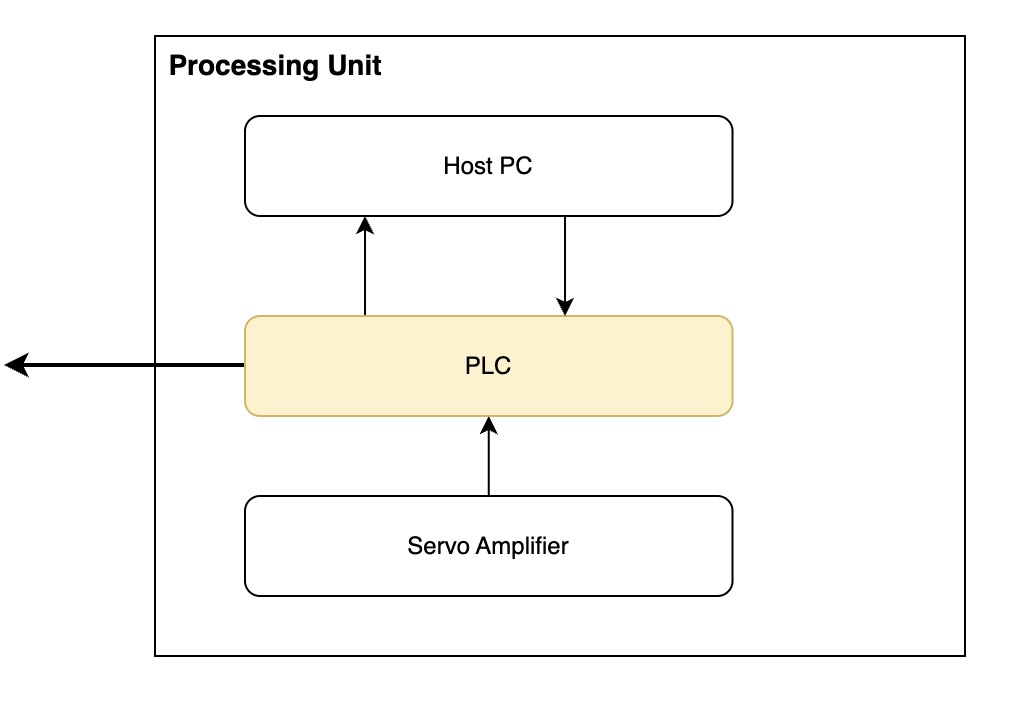
\includegraphics[width=0.65\textwidth]{images/PLC.jpg}
 \caption{PLC Subsystem}
\end{figure}

\subsubsection{Subsystem Hardware}
The PLC consists of a MELSEC Programmable Logic Controller manufactured by Mitsubishi, equipped with an integrated ethernet switch for communication with the host PC.

\subsubsection{Subsystem Operating System}
Operating on a real-time operating system (RTOS), the PLC ensures precise timing and reliable execution of control logic.

\subsubsection{Subsystem Software Dependencies}
Software tools such as GXWorks and MRConfigurator2, provided by Mitsubishi Electric, enable the programming and configuration of the PLC for control tasks.


\subsubsection{Subsystem Programming Languages}
Programming languages supported by GXWorks, including ladder logic, function block diagrams, and structured text, are utilized for developing control algorithms tailored to the application. RT ToolBox is written in MELFA BASIC VI


\subsubsection{Subsystem Data Processing}
The PLC processes sensor feedback and command signals in real-time, executing control logic to coordinate the movements of the robotic arm and additional axis. Communication with the host PC via Ethernet/IP facilitates efficient data exchange for seamless system operation.










\newpage
\section{Robot Arm Layer Subsystems}
This section consists of the robot arm, where the actual movement of the robot happens along with the application, which would be the paintball marker associated with it. The robot arm receives commands from the Controller, which gives it instructions on how it can move the joints, linear rail, and the pneumatic line for the trigger to shoot the paintball. These communication 


\subsection{Layer Hardware}
There are multiple hardware components for this layer. This layer consists of the joints that are controlled by the program in the computer. There is also pneumatic portion which controls the air that will flow through the solenoid valves. The system is also integrated with a linear rail which will control the linear movement of the entire robot arm. These systems are connected to the robot controller which controls these movements and enable communication with the controller.

\subsection{Layer Operating System}
The robot arm uses MELFA Works Operating System.

\subsection{Layer Software Dependencies}
The software dependencies include the use of RT Toolbox3 software to program the movement of the joints, GX Works software to control the PLC and a USB connection to enable the communication between the robot arm and the controller. 

\subsection{Subsystem 1}
Joints are a hardware component of the robot arm that gives the robot a specific orientation to carry out certain tasks. This will require communication from the robot controller and software, RT Toolbox3, which will give it specific orientation.

\begin{figure}[h!]
	\centering
 	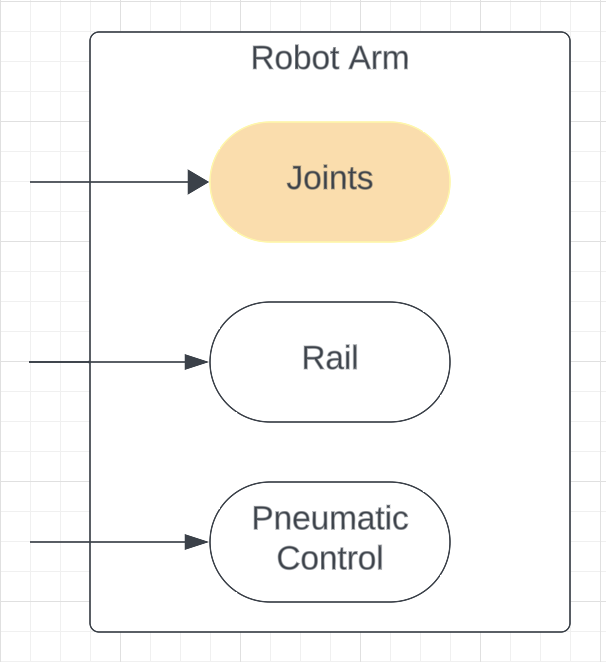
\includegraphics[width=0.60\textwidth]{images/joints.png}
 \caption{Joints Subsystem}
\end{figure}

\subsubsection{Subsystem Hardware}
This subsystem has encoders which communicates the speed of joints back to controller, so that they can adjust. They also have automatic braking system embedded into them to quickly brake if E-stops are enabled. 

\subsubsection{Subsystem Operating System}
Joints use the MELFA Works Operating System to control their orientation and movement.

\subsubsection{Subsystem Software Dependencies}
These joints require the use of RT Toolbox3 for their movement and orientation.

\subsubsection{Subsystem Programming Languages}
The programs of their movement is written in MELFA BASIC VI.

\subsubsection{Subsystem Data Structures}
Some data structures utilized by these joints are joint state and trajectory data structure which give information to the joints on where to move.

\subsubsection{Subsystem Data Processing}
We will be using the joints coordinates given in degrees in order to control their movements. They will be given in a tuple, and we will set boundaries on the limits on where the joints can move.


\subsection{Rail}
Rail is component of the RV8 robot arm which can move all the joints on a linear plane. This gives the robot arm more space to operate and more room in order to perform tasks on a wider plane. The rail receives commands from the servo amplifier which communicates with the robot controller.

\begin{figure}[h!]
	\centering
 	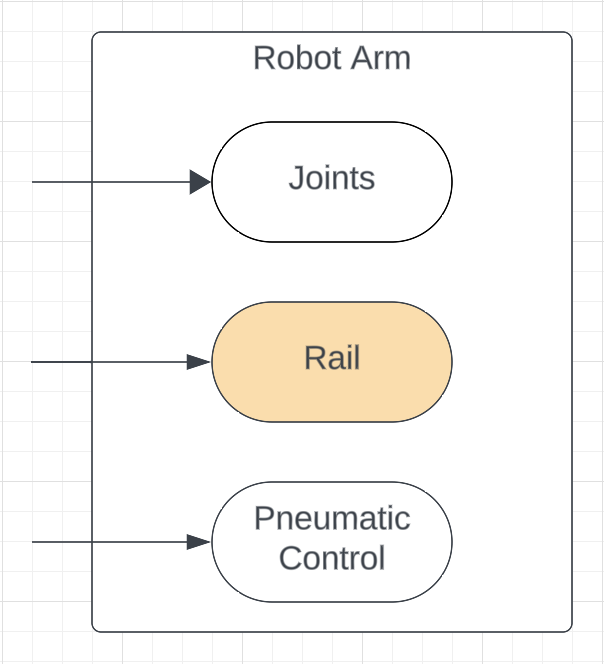
\includegraphics[width=0.60\textwidth]{images/rail.png}
 \caption{Rail Subsystem}
\end{figure}

\subsubsection{Subsystem Hardware}
This subsystem has servo motor which gives the rail its motion. The servo motor communicates with the servo amplifier. The servo motor also consists of encoders which controls the speed of the rail. It also consists of a braking system which limits it from movement when the robot arm is powered off.

\subsubsection{Subsystem Operating System}
Linear rail use the MELFA Works Operating System to control their movement.

\subsubsection{Subsystem Software Dependencies}
The rail requires RT Toolbox3 to program its movements.

\subsubsection{Subsystem Programming Languages}
The programs of their movement is written in MELFA BASIC VI.

\subsubsection{Subsystem Data Structures}
Data structures utilized by these consist of movement data structures, especially those of kinetic and dynamic structures, position, which help enable the movement of the linear rail.

\subsubsection{Subsystem Data Processing}
For data processing, the linear rail will use have a set origin, and can be configured according to the application. This will include adjusting its movement according the image that will be processed.




\subsection{Pneumatic Control}
Pneumatic system is connected to the RV8 robot and controls the air pressure that will travel through the robot. The wiring is connected to the PLC which, through the programs, will control the air pressure that will travel through the pipes. The pneumatic control will be connected through solenoid valves which will control the compressed air.

\begin{figure}[h!]
	\centering
 	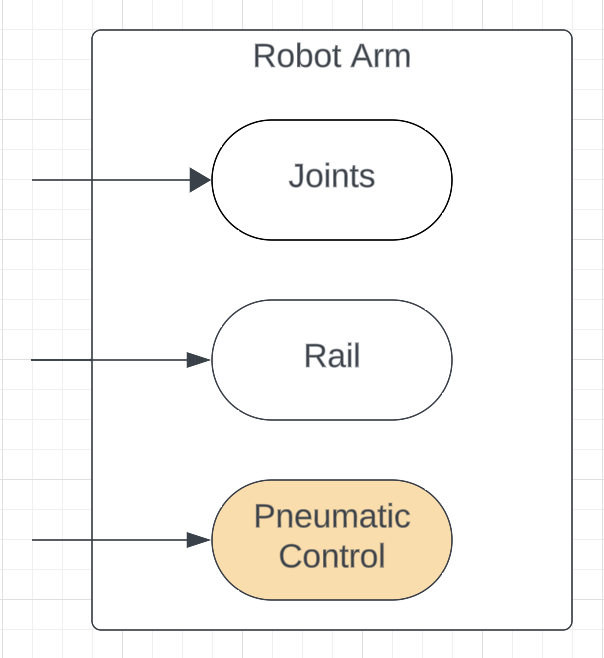
\includegraphics[width=0.60\textwidth]{images/pneumatic.png}
 \caption{Pneumatic Control Subsystem}
\end{figure}

\subsubsection{Subsystem Hardware}
This subsystem has PLC which will be programmed in order to control the compressed air, and has solenoid valves will be connected to the PLC. This will help the compressed air to trigger the paintball marker.

\subsubsection{Subsystem Operating System}
Pneumatic Control use the MELFA Works Operating System to control their movement.

\subsubsection{Subsystem Software Dependencies}
The pneumatic control requires GXWorks3 for programming

\subsubsection{Subsystem Programming Languages}
The programs of their movement is written in Ladder Logic.

\subsubsection{Subsystem Data Structures}
Data structures utilized by these consist of valve state data structures, which also consists pressure and flow data structures. These will be used in order to control the compressed air flow.

\subsubsection{Subsystem Data Processing}
For data processing, the pneumatic control will use to activate and deactivate solenoid valves. There are also going to be sensors that will transmit data regarding the proper functioning of the solenoid valves.
\newpage
\section{Indicator Layer Subsystems}
\subsection{Indicator Layer Subsystems}
The indicator layer will be responsible for the output of the system, where the indicator subsystem
consists of an industrial light tower, which displays the status of the working cell.

\begin{figure}[h!]
	\centering
 	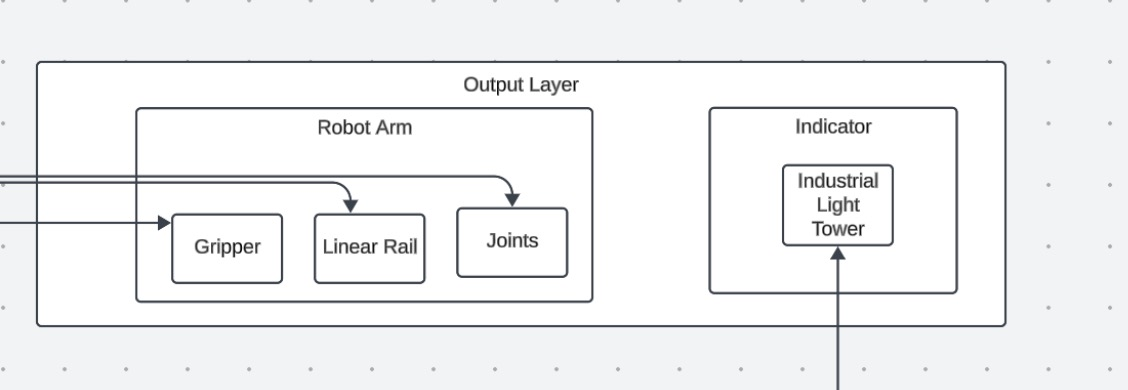
\includegraphics[width=0.60\textwidth]{images/indicator.jpg}
 \caption{Indicator Layer Subsystem}
\end{figure}

\subsubsection{Industrial Light Tower}
An industrial light tower system, typically used in a working cell or industrial setting, serves several
essential responsibilities to ensure the efficient and safe operation of the workspace. The specific responsibilities of an industrial light tower system may vary depending on the application. For our system,
it serves as an inference to the work environment as it indicates different modes with colored LEDs as
get input from the controller and outputs as LEDs.

\subsubsection{Subsystem Operating System}
No operating system required. 

\subsubsection{Subsystem Software Dependencies}
No software dependencies required by the subsystem.

\subsubsection{Subsystem Programming Languages}
No programming Language required.

\subsubsection{Subsystem Data Structures}
No data structures required. 

\subsubsection{Subsystem Data Processing}
No data processing require.



\newpage
\section{Appendix A}
\input{tex/appendix_a.tex}
\newpage

%%% References
\bibliographystyle{plain}
\bibliographystyle{reference/IEEEtran_custom}
\bibliography{reference/refs}{}

\end{document}